En esta sección vamos a hablar de las tecnologías principales que se van a utilizar en este proyecto. Se va a intentar dar una breve descripción de las mismas, ya que el objetivo no es aprender a usarlas sino decir y nombrar el porque me van a valer en este proyecto, porque he decidido esas herramientas y no otras. 

Las principales herramientas son: 

\subsubsection{Taiga}
Taiga \cite{taiga} es una herramienta que hemos nombrada anteriormente que nos permite el control de proyectos, normalmente orientado a proyectos software, de una manera sencilla, cómoda y visual. 

Taiga ofrece registrarse en su plataforma de manera gratuita. También da la posibilidad de creación de proyectos públicos o privaos como en github. Cada uno de estos proyectos te deja seleccionar si ha de seguir el modelo Kanban o Scrum, para poner la configuración por defecto del mismo. 

Una vez creado el proyecto, el tablero principal de control de proyecto, con algunas tareas añadidas queda de la siguiente manera:

\begin{figure}[H]
    \centering
    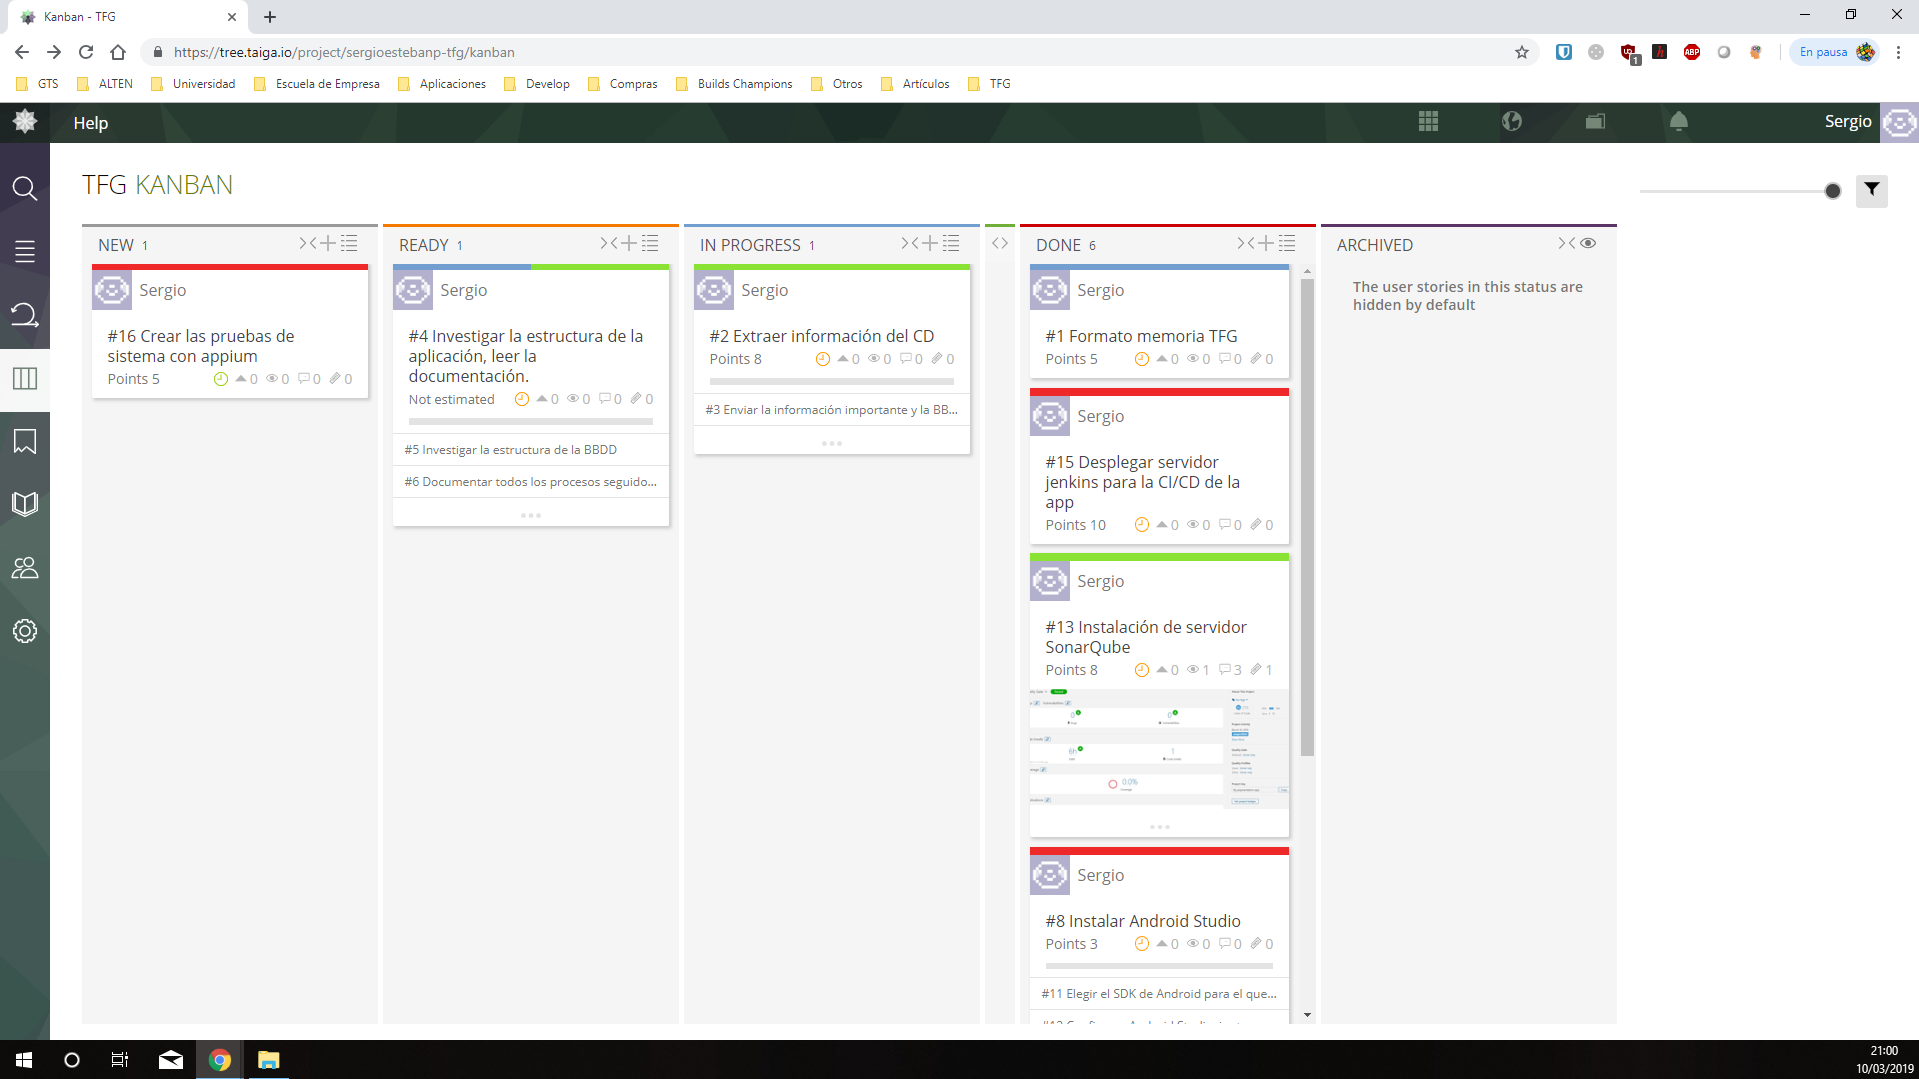
\includegraphics[scale=0.3]{imagenes/introduccion/taiga.png}
    \caption{Tablero de Taiga.io}
    \label{fig:tableroTaiga}
\end{figure}

En la figura anterior podemos ver el proyecto publico donde se ira actualizando el proceso de creación de este mismo documento y de todo el trabajo de fin de grado []. Además podemos observar las principales columnas que hemos nombrado anteriormente cuando describíamos la metodología de trabajo. 

Además del tablero principal, esta herramienta nos permite muchas mas opciones, como las siguientes: 
\begin{itemize}
    \item \textbf{Timeline}: en este apartado, podemos ver la cronología de todas las actividades realizadas en el proyecto, desde cuando se ha creado una tarea, cuando se ha actualizado el ultimo issue encontrado o cuando se ha añadido o quitado información a la wiki del proyecto. 
    \item \textbf{Backlog}: aquí podemos encontrar todas las tareas, historias de usuario y issues que hemos ido creando en el proyecto. Se presentan de forma resumida, con el estado principal, fecha de creación, etc. 
    \item \textbf{Issues}: los issues o problemas, son los diferentes problemas o bugs que nos vamos encontrando conforme el desarrollo de la aplicación se va realizando. 
    \item \textbf{Wiki}: nos proporciona una herramienta de documentación interna para el proyecto. Podemos asemejar esta wiki a Confluence \cite{confluence}, que es una herramienta de pago creada por la empresa Atlassian, para tener información y documentación en la nube. Nosotros usaremos esta wiki para anotar cosas puntuales de desarrollo o configuración. 
    \item \textbf{Members}: podemos ver a los demás miembros del equipo, en este caso solo voy a ser por lo que este apartado carece de especial importancia. 
\end{itemize}

Podemos encontrar el proyecto de este trabajo de fin de grado en la siguiente dirección \footnote{https://tree.taiga.io/project/sergioestebanp-tfg/kanban}. 

\subsubsection{SonarQube}
SonarQube \cite{sonarqube} es una herramienta que nos permite obtener métricas y medidas de la calidad de nuestro código. Nos permite obtener métricas generales de la calidad el código, a nivel de buenas y malas practicas que estamos cumpliendo, posibles vulnerabilidades junto con el nivel de criticidad de las mismas, nivel de complejidad de diversos tipos, como por ejemplo la ciclomática \footnote{La complejidad ciclotímica se mide en la cantidad de caminos individuales que se pueden recorrer en nuestro código. Cuanta menor complejidad ciclotímica mejor es la calidad del código}.

He decidido integrar SonarQube y otras tecnologías en contenedores Docker \cite{docker} En realidad no se gana demasiado dockerizando las herramientas, pero si que es verdad que permite una mayor flexibilidad, a la hora de recrear esa instancia, simplemente tenemos que copiar y pegar el bakcup de la imagen. Dockerizar los servidores en contenedores individuales es una buena medida de seguridad si la aplicación estuviera en producción y se sirvieran los servicios hacia el exterior. 

Nosotros vamos a integrar SonarQube y medir la calidad de nuestro código de 3 maneras diferentes. La primera y mas directa es en nuestro proyecto de Android Studio junto con Gradle \cite{gradle}. Ya que los proyectos de aplicaciones móviles de Android se hacen con el constructor Gradle, y Sonar (acortación de SonarQube de aquí en adelante) tiene integración con dicha herramienta, solo tenemos que crear el proyecto en el servidor previamente desplegado en docker e introducir las siguientes lineas de código en el fichero build.gradle de nuestra aplicación, mostrado en la figura \ref{fig:buildGradle}.

\begin{figure} \label{fig:buildGradle}
\lstinputlisting[style=customc]{capitulos/introduccion/codigo/build.gradle}
\caption{Configuración del fichero build.gradle}
\end{figure}

Creamos la tarea en gradle correspondiente para enviar la información a nuestro servidor de análisis y el resultado es el mostrado en la siguiente figura: 

\begin{figure}[H]
    \centering
    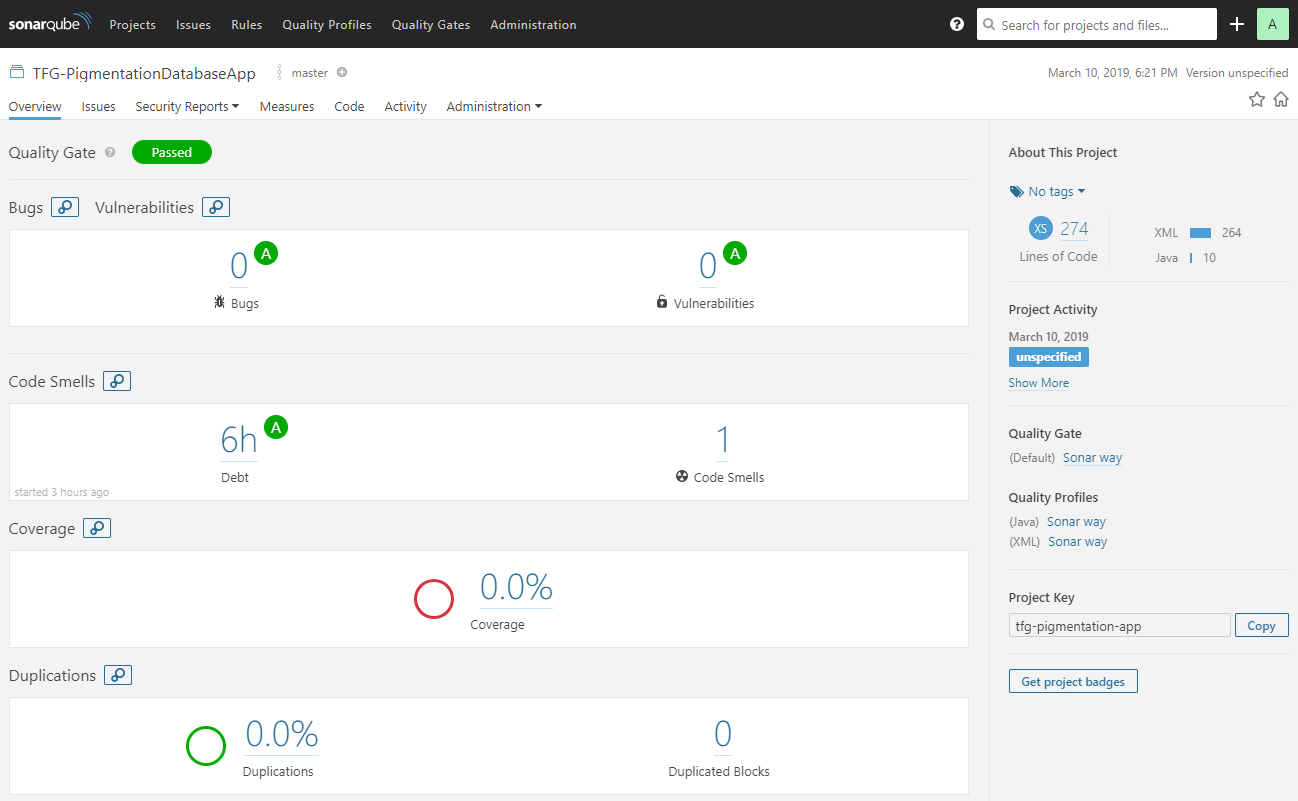
\includegraphics[scale=0.35]{imagenes/introduccion/sonarqube1.png}
    \caption{Primer análisis del código inicial generado por Android Studio}
    \label{fig:mainSonar}
\end{figure}

\begin{figure}[H]
    \centering
    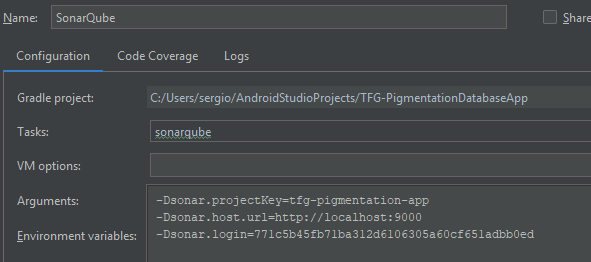
\includegraphics[scale=1]{imagenes/introduccion/sonarGradleTask.png}
    \caption{Tarea Gradle para Sonar}
    \label{fig:sonarGradleTask}
\end{figure}

Una vez tenemos estos parámetros colocados y el servidor funcionando, podemos pasar a la configuración de SonarLint.

\subsubsection{SonarLint}
SonarLint \cite{sonarlint} es un plugin para los entornos de desarrollo proporcionados por JetBrains, como Intellij IDEA o Android Studio. SonarLint nos proporciona la potencia de SonarQube pero sin tener que estar ejecutando el codigo en el servidor de manera constante. Lo que hacemos es configurar nuestro servidor de SonarQube en el plugin, y cada vez que abrimos un fichero de tipo Java, el plugin pasa el fichero por el servidor y nos devuelve los resultados de una manera muy agradable. Podemos ver un ejemplo del uso de SonarLint en la siguiente figura:

\begin{figure}[H]
    \centering
    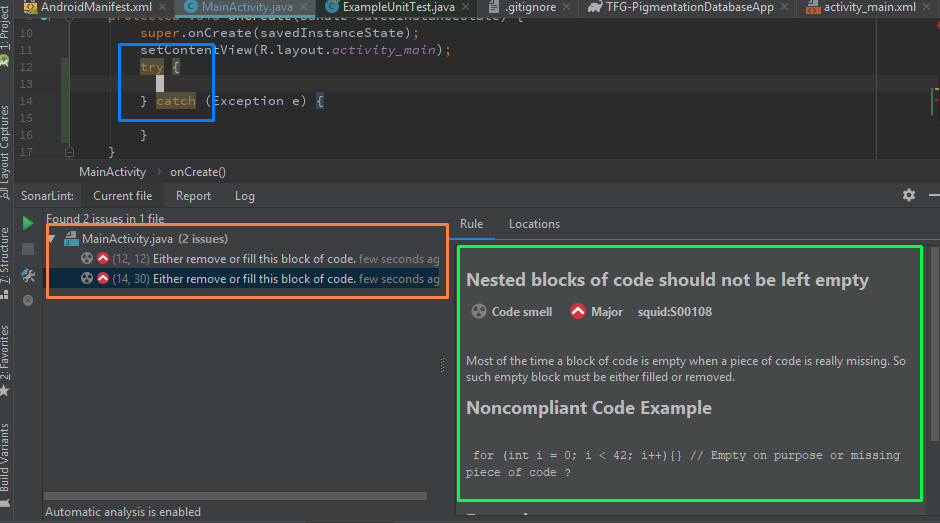
\includegraphics[scale=0.5]{imagenes/introduccion/sonarLint.png}
    \caption{SonarLint en Android Studio}
    \label{fig:sonarLinr}
\end{figure}

En el recuadro de color azul, podemos apreciar como el plugin nos muestra las vulnerabilidades de código. En el recuadro naranja nos lista todas las posibles vulnerabilidades o fallos que tiene nuestro software, y en el recuadro verde nos pone lo que significan, argumentos de porqué ese código no es de calidad y lo más importante, es que nos pone ejemplos para solucionarlo de manera sencilla y eficaz. 

\subsubsection{Jenkins}
Jenkins \cite{jenkins} es una herramienta basada en la integración continua de productos software y en el desarrollo continuo. En nuestro caso lo vamos a usar como tal. Como todo producto software, nuestra aplicación va a requerir pruebas, tanto unitarias como de otros tipos. La idea es meter toda esta suite de pruebas en jenkins e integrarla tanto con github como con sonar. Lo que vamos a hacer es definir una serie de casos de prueba, tanto a nivel unitario como test de regresión, para que cada vez que el código se vea modificado por una Pull Request (nada más allá de una solicitud de cambio), la aplicación tenga que pasar los test satisfactoriamente para comprobar que no hemos roto lo anterior. Esto es para lo que vamos a usar Jenkins principalmente. Además como Jenkins tiene muchas utilidades, también podemos integrar SonarQube para que nos notifique en caso de que en una Pull Request la calidad de nuestro código se vea afectada a peor. 

Un ejemplo de la estructura y flujo que sigue Jenkins es el siguiente:

\begin{figure}[H]
    \centering
    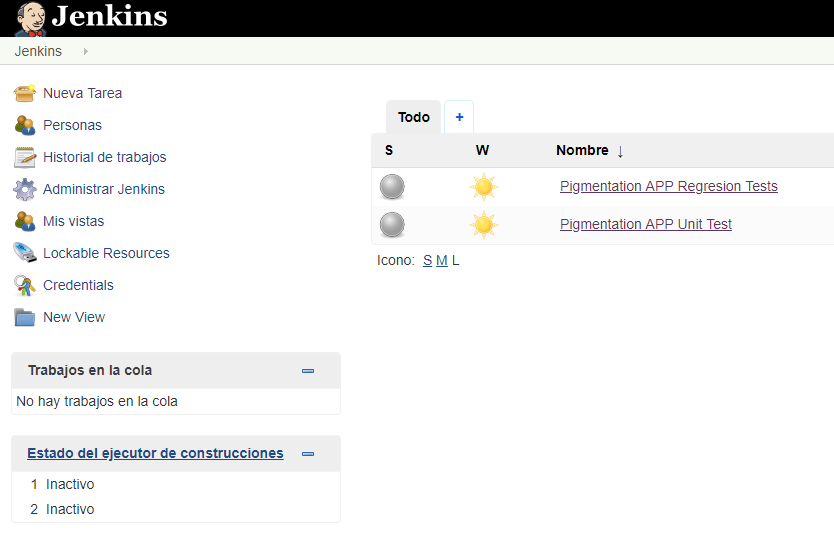
\includegraphics[scale=0.6]{imagenes/introduccion/jenkins.png}
    \caption{Flujo seguido por Jenkins}
    \label{fig:buildjenkins}
\end{figure}

En Jenkins nosotros lo que definimos son un flujo por el que pasará nuestra aplicación. En el caso de nuestra aplicación seguramente tendremos dos flujos diferentes, uno para pasar los test unitarios cada vez que hagamos una propuesta de cambio a nuestro código; y otro flujo separado que serán las pruebas de regresión. Las pruebas de regresión las haremos cuando tengamos una base de funcionamiento de la aplicación, ya que las haremos sobre la interfaz. Por ejemplo la descripción de los flujos seguidos serían:

\begin{itemize}
    \item \textbf{Pipeline ejemplo}: Obtener el código $\rightarrow$ pasar las pruebas unitaras $\rightarrow$ pasar las pruebas de calidad $\rightarrow$ generar los reportes $\rightarrow$ desplegar los cambios o dar el visto bueno.
\end{itemize}

Los flujos de Jenkins se describen mediante unos ficheros llamados Jenkinsfile, también pueden ser especificados en el propio servidor, pero no es una practica recomendable. Normalmente se integra en un archivo separado en el repositorio, precisamente para tener un seguimiento de los cambios que se hacen en el mismo. Dichos ficheros son escritos en groovy, que se basa en Java, pero simplificado. 

Un vistazo al panel general de Jenkins, es el siguiente:

\begin{figure}[H]
    \centering
    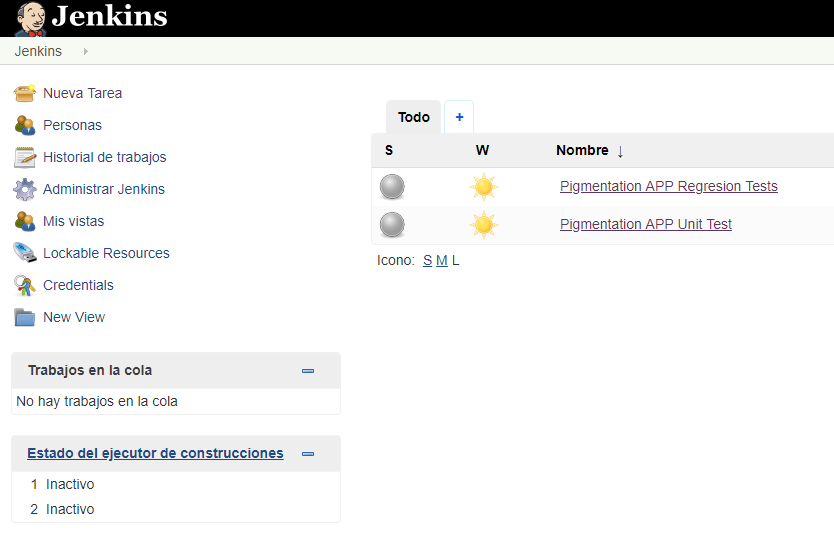
\includegraphics[scale=0.7]{imagenes/introduccion/mainJenkins.png}
    \caption{Panel General de jenkins}
    \label{fig:mainJenkins}
\end{figure}


\subsubsection{Android Studio}
Android Studio \cite{androidstudio}, no hay mucho que decir, simplemente que es un entorno de desarrollo integrado que trae todas las herramientas necesarias casi de manera nativa la la programación y testeo de aplicaciones para dispositivos multiplataforma, como pueden ser los productos del sistema operativo Android. Las principales herramientas que utilizaremos serán las ejecuciones gradle automáticas, la capacidad de simulación de un dispositivo de la familia Android de manera casi nativa, el debugger que tiene, junto con el profiler son de gran calidad desde mi punto de vista, la integración con cantidad de plugins como el ya mencionado de SonarLint o VIM son también de una calidad excelente. En general para la realización de este proyecto me he decantado por Android Studio por la centralización de las herramientas que trae el propio IDE. 

Al igual que estamos desarrollando con este IDE se pueden configurar otros como Intellij o Visual Studio Code para trabajar de manera similar. 

En mi caso voy a utilizar Android Studio por la familiaridad a la hora de trabajr con él. 

\subsubsection{Github}
Github \cite{github} es generalmente conocido (o debería serlo) para todos los desarrolladores que trabajan en el gremio. Será utilizado como gestor de versiones de código y gestor de cambios del proyecto. 
Como hemos mencionado anteriormente en la metodología (Sección \ref{sec:metodologia}), vamos a seguir un patrón para la creación de ramas y gestionar los cambios en el código. Github nos permite seguir estos patrones e implementarlos de una manera sencilla y eficaz. Además cabe destacar que Android Studio tiene integración con Github y permite de manera sencilla hacer commits, cambiar entre ramas y demás operaciones importantes. 

El repositorio de código de nuestra aplicación se encontrará en la siguiente dirección: 

\begin{quote}
    https://github.com/SergioEstebanP/TFG-PigmentationDatabaseApp
\end{quote}

\subsubsection{Overleaf}
Overleaf \cite{overleaf} es un editor de textos online que nos permite generar documentos usando \LaTeX. Por comodidad a la hora de gestionar la configuración del documento, se ha determinado usar latex como sistema de composición de textos, ya que word no ofrece las características necesarias para ello. Por lo menos no para mi. 

Algunas de las razones elegidas son:
\begin{itemize}
    \item Gestión automática de contenidos tales como figuras, tablas, títulos o secciones. 
    \item Generación y gestión fácil, automatice y simple de la bibliografía y las referencias.
    \item Facilidad para insertar formulas matemáticas en caso de que fuera necesario. 
    \item Configuración global del documento mas sencilla y flexible que en otros sistemas como word.
    \item Inadaptación de cambios gestionada por el propio sistema. 
    \item Overleaf tiene plugin para escribir utilizando los atajos de VIM. 
\end{itemize}

El enlace al proyecto de Overleaf, donde se encuentra este mismo documento es el siguiente:

\begin{quote}
https://es.overleaf.com/read/tjcbwvvdxwtq
\end{quote}

Overleaf permite la edición múltiple de documentos y además también tiene un gestor de cambios integrado. El problema es que la línea de cambios en el tiempo que guarda es relativamente pequeña, y además muestra los cambios de una manera poco intuitiva y eficaz. La ventaja frente subir el código fuente a Github es que sigue los cambios de manera automática, mientras que subiéndolo a Github hay que hacerlo manualmente. 

\subsubsection{SQLite}
SQLite \cite{sqlite} es un sistema gestor de base de datos muy sencillo, que integra Android por defecto. La idea es que la base de datos que tenemos que explotar esté integrada junto con el código de la aplicación. La base de datos parece pequeña, por lo que no ocupará nada más que unos pocos de Mega Bytes. Además, como el fichero generado para usar la aplicación es un binario, la información no será accesible al exterior. La información solo será proporcionada por la aplicación y de la manera propuesta en los capítulos posteriores. 

Como describiremos en los capítulos posteriores, una de las primeras tareas es investigar la estructura de la base de datos y exportarla a SQLite o MySQL, ya que son SGBD a los que estoy más acostumbrado y necesarios para la compatibilidad con y buena comunicación de datos con la aplicación. 